\documentclass[11pt,letterpaper]{article}
\usepackage[lmargin=1in,rmargin=1in,tmargin=1in,bmargin=1in]{geometry}
\usepackage{homework}

\usepackage{mathtools}
\DeclarePairedDelimiter\ceil{\lceil}{\rceil}
\DeclarePairedDelimiter\floor{\lfloor}{\rfloor}

% -------------------
% Content
% -------------------
\begin{document}
\homework{Solutions --- Caleb McWhorter}

% Problem 1
\problem{10} Determine if the following functions are injective, surjective, and/or bijective. Which of the functions have an inverse function? [No formal proofs required.]
        \begin{enumerate}[(a)]
        \item $f: \mathbb{R} \to [0,1]$ defined by $f(x)= \sin^2 x$.
        \item $g: [0, \frac{\pi}{2}] \to [0, 1]$ defined by $g(x)= \cos x$.
        \item $h: \mathbb{N} \to \mathbb{Z}$ given by $h(n)= 3^n$.
        \item $j: \mathbb{Z} \times \mathbb{Z} \to \mathbb{Z}$ given by $j(n, m)= (n - m + 3)^2$.
        \end{enumerate} \pspace

\sol 
\begin{enumerate}[(a)]
\item From the plot of $f(x)$, it would seem that $f(x)$ is surjective but not injective. Because $f(x)$ is not both injective and surjective, $f(x)$ is not bijective. Because $f: \mathbb{R} \to [0, 1]$ is not bijective, it does not have an inverse function. 
	\[
	\fbox{
	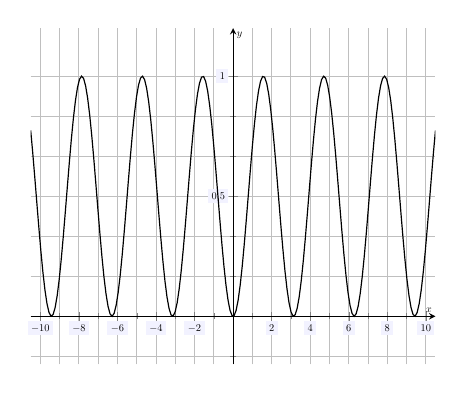
\begin{tikzpicture}[scale=0.75,every node/.style={scale=0.5}]
	\begin{axis}[
	grid=both,
	axis lines=middle,
	ticklabel style={fill=blue!5!white},
	xmin= -10.5, xmax=10.5,
	ymin= -0.2, ymax=1.2,
	xtick={-10,-8,-6,-4,-2,0,2,4,6,8,10},
	ytick={-0.2,-0.4,...,1.2},
	minor x tick num= 1,
	minor y tick num= 2,
	xlabel=\(x\),ylabel=\(y\),
	]
	\addplot[line width= 0.02cm,samples=200,domain= -10.5:10.5] ({x},{sin(deg(x))^2)}); 

	\end{axis}
	\end{tikzpicture}
	}
	\] 
To see this directly, observe that $0, \pi \in \mathbb{R}$, $f(0)= \sin^2(0)= 0$, and $f(\pi)= \sin^2(\pi)= 0$. Because $f(0)= f(\pi)$ and $0 \neq \pi$, we know that $f(x)$ is not injective. Alternatively, $f(x)$ is not injective because there is a horizontal line which intersects the graph of $f(x)$ more than once, e.g. the horizontal line $y= 1$. Alternatively, observe that $f(x)$ is surjective because every horizontal line $y= c$, where $c \in [0, 1]$, intersects the graph of $f(x)$ at least once. We know that $\arcsin x$ is defined when $-1 \leq x \leq 1$. Let $y \in [0, 1]$ and define $x:= \arcsin(\sqrt{y})$ (observe that $\sqrt{y}$ is defined because $y \geq 0$ and $\arcsin(\sqrt{y})$ is defined because $-1 \leq \sqrt{y} \leq 1$). Then $f(x)= f(\arcsin(\sqrt{y}))= \big( \sin( \arcsin( \sqrt{y} ) ) \big)^2= (\sqrt{y})^2= y$. Therefore, $f(x)$ is surjective. \pspace

\item From the plot of $g(x)$, it would seem that $g(x)$ is injective and surjective. Because $g(x)$ is both injective and surjective, it is bijective. Because $g: [0, \frac{\pi}{2}] \to [0, 1]$ is bijective, we know that $g(x)$ has an inverse function, i.e. $g^{-1}: [0, 1] \to [0, \frac{\pi}{2}]$ exists. In fact, the inverse is $\arccos x: [0, 1] \to [0, \frac{\pi}{2}]$. 
	\[
	\fbox{
	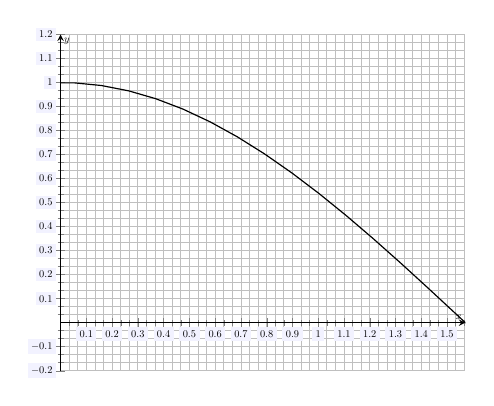
\begin{tikzpicture}[scale=0.75,every node/.style={scale=0.5}]
	\begin{axis}[
	grid=both,
	axis lines=middle,
	ticklabel style={fill=blue!5!white},
	xmin= 0, xmax=pi/2,
	ymin= -0.2, ymax=1.2,
	xtick={0,0.1,...,1.6},
	ytick={-0.2,-0.1,...,1.2},
	minor x tick num= 2,
	minor y tick num= 2,
	xlabel=\(x\),ylabel=\(y\),
	]
	\addplot[line width= 0.02cm,samples=200,domain= -10.5:10.5] ({x},{cos(deg(x))}); 

	\end{axis}
	\end{tikzpicture}
	}
	\] 
We can see these facts directly. To see that $g(x)$ is injective, observe that every horizontal line $y= c \in [0, 1]$ intersects the graph of $g(x)$ at most once. Alternatively, recall that $\arccos x$ is defined for $x \in [-1, 1]$ and produces values in $[0, \pi]$. Let $x, y \in [0, \frac{\pi}{2}]$ and suppose that $g(x)= g(y)$, i.e. $\cos(x)= \cos(y)$. But then $x= \arccos \big(\cos(x) \big)= \arccos \big(\cos(y) \big)= y$, where we have used the fact that $x, y \in [0, \frac{\pi}{2}]$. Therefore, $g(x)$ is injective. To see that $g(x)$ is surjective, observe that every horizontal line $y= c \in [0, 1]$ intersects the graph of $g(x)$ at least once. Alternatively, recall that $g(x)= \cos x$ is continuous. We know that $g(0)= \cos(0)= 1$ and $g(\frac{\pi}{2})= \cos(\frac{\pi}{2})= 0$. By the Intermediate Value Theorem, for any $y \in [0, 1]$, there exists $x \in [0, \frac{\pi}{2}]$ such that $g(x)= y$. But then $g(x)$ is surjective. \pspace

\item We can plot a few values for this function. From this plot it seems that $h(n)$ is injective but not surjective. Because $h(n)$ is not both injective and surjective, $h(n)$ is not bijective. Because $h: \mathbb{N} \to \mathbb{Z}$ is not bijective, it does not have an inverse function. 
	\[
	\fbox{
	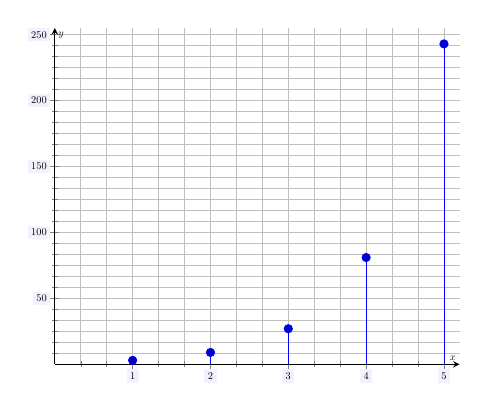
\begin{tikzpicture}[scale=0.75,every node/.style={scale=0.5}]
	\begin{axis}[
	grid=both,
	axis lines=middle,
	ticklabel style={fill=blue!5!white},
	xmin= 0, xmax=5.2,
	ymin= 0, ymax=255,
	xtick={0,1,...,5},
	ytick={0,50,...,250},
	minor x tick num= 2,
	minor y tick num= 5,
	xlabel=\(x\),ylabel=\(y\),
	]
	\addplot+[ycomb,domain=0:10, samples at={1,2,3,4,5}, blue] {3^x};
	\end{axis}
	\end{tikzpicture}
	}
	\] 
We can see these facts directly. To see that $h: \mathbb{N} \to \mathbb{Z}$ is not surjective, observe that not every horizontal line $y= z \in \mathbb{Z}$ intersects the graph of the function. For instance, the lines $y= 2$ and $y= -5$ do not intersect the graph of $h(n)$. Alternatively, consider $0 \in \mathbb{Z}$. Because $h(n) > 0$, there does not exist $n \in \mathbb{N}$ such that $h(n)= 0$. Therefore, $h(n)$ is not surjective. To see that $h(n)$ is injective, observe that every horizontal line $y= z \in \mathbb{Z}$ intersects the graph of $h(n)$ at most once. Alternatively, suppose that $n, m \in \mathbb{N}$ with $n \neq m$. Without loss of generality, assume that $n < m$. Because $\widetilde{h}(x)= 3^x$ has the property that $\widetilde{h}'(x)= 3^x \ln(3) > 0$, we know that $\widetilde{h}(x)$ is increasing. But then $h(n)$ is increasing. But then because $n < m$, $h(n)= 3^n < 3^m= h(m)$. Therefore, if $n \neq m$, we know $g(n) \neq g(m)$. This shows that $h(n)$ is injective. \pspace

\item Though we cannot (usefully) plot $j(n, m)$, we can still easily determine that $j$ is neither injective nor surjective. Because $j$ is not both injective and surjective, $j$ is not bijective. Because $j: \mathbb{Z} \times \mathbb{Z} \to \mathbb{Z}$ is not bijective, it does not have an inverse function. To see that $j$ is not injective, observe that $(0, 0), (1, 1) \in \mathbb{Z} \times \mathbb{Z}$, $j(0, 0)= (0 - 0 + 3)^2= 3^2= 9$, and $j(1, 1)= (1 - 1 + 3)^2= 3^2= 9$. Because $(0, 0) \neq (1, 1)$ but $j(0, 0)= j(1, 1)$, we know that $j$ is not injective. To see that $j$ is not surjective, observe that $n - m + 3 \in \mathbb{Z}$ because $n, m \in \mathbb{Z}$. But then $(n - m + 3)^2 \geq 0$. Therefore, there exist no $n, m \in \mathbb{Z}$ such that $(n - m + 3)^2= -1$. But then there exists no $(n, m) \in \mathbb{Z} \times \mathbb{Z}$ such that $j(n, m)= -1$. Therefore, $j$ is not surjective. 
\end{enumerate}



\newpage



% Problem 2
\problem{10} Show that the function $f: \mathbb{R} \setminus \{ -1 \} \to \mathbb{R} \setminus \{ 3 \}$ given by $f(x)= \dfrac{3x - 5}{x + 1}$ is a bijection. Explain why this implies $f$ is invertible and then find the inverse for $f(x)$. \pspace

\sol To show that $f: \mathbb{R} \setminus \{ -1 \} \to \mathbb{R} \setminus \{ 3 \}$ is bijective, we need to prove that $f$ is both injective and surjective. To see that $f$ is injective, let $x, y \in \mathbb{R} \setminus \{ 1 \}$ and suppose that $f(x)= f(y)$. We need to show $x= y$. But $f(x)= f(y)$ implies\dots
	\[
	\begin{gathered}
	f(x)= f(y) \\
	\dfrac{3x - 5}{x + 1}= \dfrac{3y - 5}{y + 1} \\
	(3x - 5)(y + 1)= (3y - 5)(x + 1) \\
	3xy + 3x - 5y - 5= 3xy + 3y - 5x - 5 \\
	3x - 5y= 3y - 5x \\
	8x= 8y \\
	x= y
	\end{gathered}
	\]
Therefore, $f$ is injective. \pspace

To see that $f$ is surjective, suppose that $y \in \mathbb{R} \setminus \{ 3 \}$. We need to show there exists $x \in \mathbb{R} \setminus \{ -1 \}$ such that $f(x)= y$. Because $y \neq 3$, we can define $x:= \frac{y + 5}{3 - y}$. We need to show that $x \neq -1$. If $x= -1$, then
	\[
	\begin{gathered}
	x= -1 \\[0.1cm]
	\dfrac{y + 5}{3 - y}= -1 \\[0.1cm]
	y + 5= y - 3 \\[0.1cm]
	5= -3
	\end{gathered}
	\]
which is impossible. Therefore, $x \neq -1$. Observe\dots
	\[
	f(x)= \dfrac{3x - 5}{x + 1}= \dfrac{3 \cdot \frac{y + 5}{3 - y} - 5}{\frac{y + 5}{3 - y} + 1}= \dfrac{\frac{3y + 15}{3 - y} - \frac{15 - 5y}{3 - y}}{\frac{y + 5}{3 - y} + \frac{3 - y}{3 - y}}= \dfrac{\frac{8y}{3 - y}}{\frac{8}{3 - y}}= \dfrac{8y}{8}= y 
	\]
Therefore, $f$ is surjective. \pspace

Because $f$ is both injective and surjective, $f: \mathbb{R} \setminus \{ -1 \} \to \mathbb{R} \setminus \{ 3 \}$ is a bijection. Therefore, $f^{-1}: \mathbb{R} \setminus \{ 3 \} \to \mathbb{R} \setminus \{ -1 \}$ exists. We can find it by interchanging the roles of $x$ and $y$ and solving for $y$:
	\[
	\begin{gathered}
	x= \dfrac{3y - 5}{y + 1} \\[0.1cm]
	x(y + 1)= 3y - 5 \\[0.1cm]
	xy + x= 3y - 5 \\[0.1cm]
	xy - 3y= -x - 5 \\[0.1cm]
	y(x - 3)= -x - 5 \\[0.1cm]
	y= \dfrac{-x - 5}{x - 3} \\[0.1cm]
	y= \dfrac{x + 5}{3 - x}
	\end{gathered}
	\]
Therefore, $f^{-1}: \mathbb{R} \setminus \{ 3 \} \to \mathbb{R} \setminus \{ -1 \}$\footnote{We need prove that $f^{-1}$ has the correct domain and codomain. Because $f: \mathbb{R} \setminus \{ -1 \} \to \mathbb{R} \setminus \{ 3 \}$, we need to prove $f^{-1} \colon \mathbb{R} \setminus \{ 3 \} \to \mathbb{R} \setminus \{ -1 \}$. Clearly, $f^{-1}$ is defined on $\mathbb{R} \setminus \{ 3 \}$. We need to prove that $\text{im } f^{-1} \subseteq \mathbb{R} \setminus \{ -1 \}$. Clearly, $\text{im } f^{-1} \subseteq \mathbb{R}$. So we only need show that $-1 \notin \text{im } f^{-1}$, i.e. $f^{-1}(x) \neq -1$ for all $x$. If $f^{-1}(x)= -1$ for some $x$, then $\frac{x + 5}{3 - x}= -1$. But this implies $x + 5= x - 3$, which forces $5= -3$, which is impossible. Therefore, $f^{-1}(x) \neq -1$ for all $x$. This proves that $-1 \notin \text{im } f$ so that $\text{im } f^{-1} \subseteq \mathbb{R} \setminus \{ -1 \}$. This proves we can allow the codomain to be $\mathbb{R} \setminus \{ -1 \}$.} is given by $f^{-1}(x)= \dfrac{x + 5}{3 - x}$.\footnote{In fact, finding $f^{-1}$ was how we found how to define $x$ given $y$ in the proof of surjectivity.} \pspace

We can easily verify that this is indeed the inverse:
	\[
	\begin{aligned}
	(f \circ f^{-1})(x)&= f \big( f^{-1}(x) \big) \qquad\qquad& (f^{-1} \circ f)(x)&= f^{-1} \big( f(x) \big) \\[0.1cm]
	&= f \left( \dfrac{x + 5}{3 - x} \right) & &= f^{-1} \left( \dfrac{3x - 5}{x + 1} \right) \\[0.1cm]
	&= \dfrac{3 \cdot \frac{x + 5}{3 - x} - 5}{\frac{x + 5}{3 - x} + 1} & &= \dfrac{\frac{3x - 5}{x + 1} + 5}{3 - \frac{3x - 5}{x + 1}} \\[0.1cm]
	&= \dfrac{\frac{3x + 15}{3 - x} - \frac{15 - 5x}{3 - x}}{\frac{x + 5}{3 - x} + \frac{3 - x}{3 - x}} & &= \dfrac{\frac{3x - 5}{x + 1} + \frac{5x + 5}{x + 1}}{\frac{3x + 3}{x + 1} - \frac{3x - 5}{x + 1}} \\[0.1cm]
	&= \dfrac{\frac{8x}{3 - x}}{\frac{8}{3 - x}} & &= \dfrac{\frac{8x}{x + 1}}{\frac{8}{x + 1}} \\[0.1cm]
	&= \dfrac{8x}{8} & &= \frac{8x}{8} \\[0.1cm]
	&= x & &= x
	\end{aligned}
	\]



\newpage



% Problem 3
\problem{10} Let $S \subseteq \mathbb{R}$ and $f, g: S \to \mathbb{R}$ be monotone increasing functions. 
        \begin{enumerate}[(a)]
        \item Prove that $f + g$ is a monotone increasing function. 
        \item If $f$ and $f + g$ are increasing on $S$, then is $g$ necessarily increasing on $S$? Prove this statement or give a counterexample. 
        \end{enumerate} \pspace

\sol 
\begin{enumerate}[(a)]
\item Recall that a function $\phi: \mathbb{R} \to \mathbb{R}$ is monotone increasing if for all $x, y \in \mathbb{R}$ with $x < y$, then $\phi(x) \leq \phi(y)$. Assume that $f, g: S \to \mathbb{R}$ are monotone increasing functions. But then if $x, y \in S$ with $x < y$, we know that $f(x) \leq f(y)$ and $g(x) \leq g(y)$. \pspace

We need to show that $(f + g)(x)$ is monotone increasing; that is, we need to show that if $x < y$, then $(f + g)(x) \leq (f + g)(y)$. Observe\dots
	\[
	(f + g)(x)= f(x) + g(x) \leq f(y) + g(x) \leq f(y) + g(y)= (f + g)(y) 
	\]
Therefore, $(f + g)(x) \leq (f + g)(y)$ so that $f + g$ is monotone increasing. \pspace

\item Recall that a function $\phi: \mathbb{R} \to \mathbb{R}$ is increasing if for all $x, y \in \mathbb{R}$ with $x < y$, then $\phi(x) < \phi(y)$. Suppose that $f, f + g: S \to \mathbb{R}$ are increasing functions. It need not be the fact that $g$ is increasing on $S$. \pspace

For example, let $S= [0, \infty)$, $f(x)= x^2 + x$, and $g(x)= -x$. Observe that $(f + g)(x)= f(x) + g(x)= (x^2 + x) + (-x)= x^2$. Because $f'(x)= 2x + 1 \geq 0$ on $[0, \infty)$ and $(f + g)'(x)= 2x \geq 0$ on $[0, \infty)$. Both $f$ and $f + g$ are clearly increasing on $[0, \infty)$. However, $g(x)= -x$ is clearly decreasing on $[0, \infty)$. 
\end{enumerate}



\newpage



% Problem 4
\problem{10} Let $f: X \to Y$ and let $A, B \in \mathcal{P}(X)$. 
        \begin{enumerate}[(a)]
        \item Prove that $f(A \cup B)= f(A) \cup f(B)$. 
        \item Is it true that $f(A \cap B)= f(A) \cap f(B)$? Prove or give a counterexample. 
        \end{enumerate} \pspace

\sol 
\begin{enumerate}[(a)]
\item To prove $f(A \cup B)= f(A) \cup f(B)$, we need to prove that $f(A \cup B) \subseteq f(A) \cup f(B)$ and $f(A) \cup f(B) \subseteq f(A \cup B)$. \pspace

$f(A \cup B) \subseteq f(A) \cup f(B)$: Let $y \in f(A \cup B)$. We want to show that $y \in f(A) \cup f(B)$. Because $y \in f(A \cup B)$, there exists $x \in A \cup B$ such that $f(x)= y$. Because $x \in A \cup B$, we know that $x \in A$ or $x \in B$. We consider both cases.
	\begin{enumerate}
	\item[] Case I, $x \in A$: If $x \in A$, then $x \in A$ and $f(x)= y$ so that $y \in f(A)$. But then $y \in f(A) \cup f(B)$. 
	\item[] Case II, $x \in B$: If $x \in B$, then $x \in B$ and $f(x)= y$ so that $y \in f(B)$. But then $y \in f(A) \cup f(B)$. 
	\end{enumerate}
Therefore, if $y \in f(A \cup B)$, then $y \in f(A) \cup f(B)$. This proves that $f(A \cup B) \subseteq f(A) \cup f(B)$. \pspace

$f(A) \cup f(B) \subseteq f(A \cup B)$: Let $y \in f(A) \cup f(B)$: Let $y \in f(A) \cup f(B)$. We want to show that $y \in f(A \cup B)$. Because $y \in f(A) \cup f(B)$, we know that $y \in f(A)$ or $y \in f(B)$. We consider both cases:
	\begin{enumerate}
	\item[] Case I, $y \in f(A)$: If $y \in f(A)$, then there exists $x \in A$ such that $f(x)= y$. Because $x \in A$, we know that $x \in A \cup B$. But then because $x \in A \cup B$ and $f(x)= y$, we know that $y \in f(A \cup B)$. 
	\item[] Case II, $y \in f(B)$: If $y \in f(B)$, then there exists $x \in B$ such that $f(x)= y$. Because $x \in B$, we know that $x \in A \cup B$. But then because $x \in A \cup B$ and $f(x)= y$, we know that $y \in f(A \cup B)$. 
	\end{enumerate}
But then if $y \in f(A) \cup f(B)$, then $y \in f(A \cup B)$. Therefore, $f(A) \cup f(B) \subseteq f(A \cup B)$. \pspace

Therefore, because $f(A \cup B) \subseteq f(A) \cup f(B)$ and $f(A) \cup f(B) \subseteq f(A \cup B)$, we know that $f(A \cup B)= f(A) \cup f(B)$. \pspace


\item No, generally, we only know that $f(A \cap B) \subseteq f(A) \cap f(B)$. [Try proving this!] The other inclusion need not hold, i.e. there may be elements of $f(A) \cap f(B)$ that may not be elements of $f(A \cap B)$. This is because there could be elements only in $A$ and $B$, i.e. $a \in A \setminus B$ and $b \in B \setminus A$ (hence, $a, b \notin A \cap B$), such that $f(a)= f(b)$. For instance, consider the function $f(x)$ given by the diagram below. 
	\[
	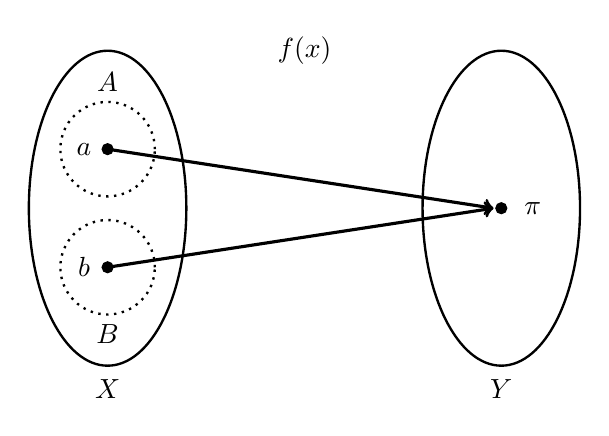
\begin{tikzpicture}
	\node at (2.5,2) {$f(x)$};
	% Ellipses
	\draw[line width=0.03cm] (0,0) circle (1 and 2);
	\draw[line width=0.03cm] (5,0) circle (1 and 2);
	
	\draw[line width=0.03cm,dotted] (0,0.75) circle (0.6 and 0.6);
	\draw[line width=0.03cm,dotted] (0,-0.75) circle (0.6 and 0.6);
	
	% Nodes
	\draw[fill=black] (0,0.75) circle (0.07);
	\draw[fill=black] (0,-0.75) circle (0.07);
	
	\draw[fill=black] (5,0) circle (0.07);
	
	% Arrow
	\draw[line width=0.04cm,->] (0,0.75) -- (4.9,0);
	\draw[line width=0.04cm,->] (0,-0.75) -- (4.9,0);
	
	% Labels
	\node at (-0.3,0.75) {$a$};
	\node at (-0.3,-0.75) {$b$};
	
	\node at (0,1.6) {$A$};
	\node at (0,-1.6) {$B$};
	
	\node at (5.4,0) {$\pi$};
	
	\node at (0,-2.3) {$X$};
	\node at (5,-2.3) {$Y$};
	\end{tikzpicture}
	\]
That is, let $f: X \to Y$ be the function given by $f(a)= \pi$ and $f(b)= \pi$. Define $A= \{ a \}$ and $B= \{ b \}$. Clearly, $A \cap B= \varnothing$. Therefore, $f(A \cap B)= f(\varnothing)= \varnothing$. Moreover, $f(A)= \{ f(x) \colon x \in A \}= \{ f(a) \}= \{ \pi \}$ and $f(B)= \{ f(x) \colon x \in B \}= \{ f(b) \}= \{ \pi \}$. But then $f(A) \cap f(B)= \{ \pi \} \cap \{ \pi \}= \{ \pi \}$. While we have $f(A \cap B)= \varnothing \subseteq \{ \pi \}= f(A) \cap f(B)$, we do not have $f(A \cap B)= f(A) \cap f(B)$. 
\end{enumerate}



\newpage



% Problem 5
\problem{10} Let $f: X \to Y$ and $A, B \subseteq Y$. Prove that $f^{-1}(A \cap B)= f^{-1}(A) \cap f^{-1}(B)$. \pspace

\sol To prove $f^{-1}(A \cap B)= f^{-1}(A) \cap f^{-1}(B)$, we need to prove that $f^{-1}(A \cap B) \subseteq f^{-1}(A) \cap f^{-1}(B)$ and $f^{-1}(A) \cap f^{-1}(B) \subseteq f^{-1}(A \cap B)$. \pspace

$f^{-1}(A \cap B) \subseteq f^{-1}(A) \cap f^{-1}(B)$: Let $x \in f^{-1}(A \cap B)$. We need to show that $x \in f^{-1}(A) \cap f^{-1}(B)$. Because $x \in f^{-1}(A \cap B)$, we know that $f(x) \in A \cap B$. But then $f(x) \in A$, which implies $x \in f^{-1}(A)$. Similarly, because $f(x) \in A \cap B$, we know that $f(x) \in B$, which implies $x \in f^{-1}(B)$. Because $x \in f^{-1}(A)$ and $x \in f^{-1}(B)$, we know $x \in f^{-1}(A) \cap f^{-1}(B)$. But then if $x \in f^{-1}(A \cap B)$, then $x \in f^{-1}(A) \cap f^{-1}(B)$. Therefore, $f^{-1}(A \cap B) \subseteq f^{-1}(A) \cap f^{-1}(B)$. \pspace

$f^{-1}(A) \cap f^{-1}(B) \subseteq f^{-1}(A \cap B)$: Let $x \in f^{-1}(A) \cap f^{-1}(B)$. We need to show that $x \in f^{-1}(A \cap B)$. Because $x \in f^{-1}(A) \cap f^{-1}(B)$, we know that $x \in f^{-1}(A)$, which implies that $f(x) \in A$. Similarly, because $x \in f^{-1}(A) \cap f^{-1}(B)$, we know that $x \in f^{-1}(B)$, which implies that $f(x) \in B$. Therefore, because $f(x) \in A$ and $f(x) \in B$, we know that $f(x) \in A \cap B$. This implies that $x \in f^{-1}(A \cap B)$. But then if $x \in f^{-1}(A) \cap f^{-1}(B)$, then $x \in f^{-1}(A \cap B)$. Therefore, $f^{-1}(A) \cap f^{-1}(B) \subseteq f^{-1}(A \cap B)$. \pspace

Therefore, because $f^{-1}(A \cap B) \subseteq f^{-1}(A) \cap f^{-1}(B)$ and $f^{-1}(A) \cap f^{-1}(B) \subseteq f^{-1}(A \cap B)$, we know $f^{-1}(A \cap B)= f^{-1}(A) \cap f^{-1}(B)$. 



\newpage



% Problem 6
\problem{10} For each of the following, find a function $f: \mathbb{N} \to \mathbb{Z}$ with the following properties:
        \begin{enumerate}[(a)]
        \item $f$ is injective but not surjective
        \item $f$ is surjective but not injective
        \item $f$ is neither surjective nor injective
        \item $f$ is a bijection
        \end{enumerate} \pspace

\sol There are infinitely many possible solutions. Here is a collection of possible solutions: 

\begin{enumerate}[(a)]
\item Let $f: \mathbb{N} \to \mathbb{Z}$ be given by $f(n)= n$. Clearly, $f$ is injective because if $f(n)= f(m)$, then $n= f(n)= f(m)= m$, so that $n= m$. Therefore, $f$ is injective. But $f$ is not surjective. Because $n \in \mathbb{N}$, we know that $n \geq 0$. But then $f(n) \geq 0$ for all $n$. But then $f(n) \neq -1$ for all $n \in \mathbb{N}$. Therefore, $f$ is not surjective. \pspace

\item Let $g: \mathbb{N} \to \mathbb{Z}$ be the bijection in (d)---no one said parts had to or should be done in order, i.e.
	\[
	g(n)= 
	\begin{cases}
	0, & n= 1 \\
	\frac{n}{2}, & n \text{ is even} \\
	-\frac{n + 1}{2}, & n \text{ is odd}
	\end{cases}
	\]
From (d), we know that $g$ is a bijection. Suppose we construct a surjection $h: \mathbb{N} \to \mathbb{N}$ that is not injective. We know that $g \circ h: \mathbb{N} \to \mathbb{Z}$ will be a surjection because the composition of surjective functions is surjective. But because $h$ is not injective, there exists $n, m \in \mathbb{N}$ with $n \neq m$ but $h(n)= h(m)$. Define $N:= h(n)= h(m)$. Then $(g \circ h)(n)= g \big (h (n) \big)= g(N)$ and $(g \circ h)(m)= g \big( h(m) \big)= g(N)$ so that $(g \circ h)(n)= (g \circ h)(m)$ but $n \neq m$. Thus, $g \circ h$ would not be injective. It remains to construct a surjection $h: \mathbb{N} \to \mathbb{N}$ that is not an injection. Let $h: \mathbb{N} \to \mathbb{N}$ be given by\dots
	\[
	h(n)=
	\begin{cases}
	\frac{n}{2}, & n \text{ even} \\
	\frac{n + 1}{2}, & n \text{ odd}
	\end{cases}
	\]
The function $h$ maps the even positive integers to $1, 2, 3, \ldots$ and maps the odd even integers to $1, 2, 3, \ldots$. To see that $h$ is not injective, observe that $h(1)= \frac{1 + 1}{2}= \frac{2}{2}= 1$ and $h(2)= \frac{2}{2}= 1$. Obviously $1 \neq 2$ but $h(1)= h(2)$, so that $h$ is not injective. It only remains to show that $h$ is surjective. Let $n \in \mathbb{N}$. We want to show there exists $m \in \mathbb{N}$ such that $h(m)= n$. Observe that $2n \in \mathbb{N}$ is even. Defining $m:= 2n$, we have $h(m)= \frac{m}{2}= \frac{2n}{2}= n$. But then for all $n \in \mathbb{N}$, there exists $m \in \mathbb{N}$ such that $h(m)= n$. Therefore, $h$ is surjective. \pspace

Now define $f:= g \circ h: \mathbb{N} \to \mathbb{Z}$, i.e. $f(n):= g \big( h(n) \big)$. We know that $f$ is surjective (because it is the composition of surjective functions is surjective) and that $f$ is not injective (because $h$ is not injective). But then $f: \mathbb{N} \to \mathbb{Z}$ is a surjection that is not injective. One can even give $f$ explicitly using the value of $n$ modulo $4$\footnote{The value of $h$ at $n$ depends upon the parity of $n$. But then the out $h(n)$ may have different parity than $n$, which is then input into $g$ whose output depends upon the parity of its input. For instance, if $n$ is even then $h(n)= \frac{n}{2}$, which may be even, e.g. $n= 8$, or odd, e.g. $n= 6$. One would then only use the `$\frac{n}{2}$' definition of $h$ and the $\frac{n}{2}$ definition of $g$ if $n$ were divisible by $2$ at least twice, i.e. divisible by four.}
	\[
	f(n)= 
	\begin{cases}
	\dfrac{n}{4}, & n \equiv 0 \mod 4 \\[0.3cm]
	-\dfrac{n - 1}{4}, & n \equiv 1 \mod 4 \\[0.3cm]
	-\dfrac{n - 2}{4}, & n \equiv 2 \mod 4 \\[0.3cm]
	\dfrac{n + 1}{4}, & n \equiv 3 \mod 4
	\end{cases}
	\]

\item Let $f: \mathbb{N} \to \mathbb{Z}$ be given by $f(n)= 0$ for all $n \in \mathbb{N}$. Clearly, $f$ is not injective because $f(1)= f(2)= 0$ but $1 \neq 2$. Furthermore, $f$ is not surjective because there is no $n \in \mathbb{N}$ such that $f(n)= 1$. \pspace

\item We will construct a function that will `count through' $\mathbb{Z}$ in the following way: $0, 1, -1, 2, -2, 3, -3, \dots$. For now, we shall focus on the sequence $1, -1, 2, -2, 3, -3, \dots$. We will create a map that assigns values in $\mathbb{N}$ to these values in the order. A table may be helpful: \par
	\begin{table}[ht]
	\centering
	\begin{tabular}{c|rrrrrrrrr}
	$n$ & $1$ & $2$ & $3$ & $4$ & $5$ & $6$ & $7$ & $8$ & $\cdots$ \\
	$f(n)$ & $1$ & $-1$ & $2$ & $-2$ & $3$ & $-3$ & $4$ & $-4$ & $\cdots$
	\end{tabular}
	\end{table} \par
Letting $f(1)= 0$ and shifting each of the outputs one spot to the right in the table above gives a `valid' description of a bijective function. However, we can be more concrete. Observe that the even integers are assigned to the negation of half their value, i.e. $-n/2$. Using this as a `hint' for the odd integers, observe that the odd integers are mapped to half of one less than their value, i.e. $(n - 1)/2$. If we want to include $0$, we can simply `shift' everything up, insert $0$, and use the same idea as above. 
 \par
	\begin{table}[ht]
	\centering
	\begin{tabular}{c|rrrrrrrrr}
	$n$ & $1$ & $2$ & $3$ & $4$ & $5$ & $6$ & $7$ & $8$ & $\cdots$ \\
	$f(n)$ & $0$ & $1$ & $-1$ & $2$ & $-2$ & $3$ & $-3$ & $4$ & $\cdots$
	\end{tabular}
	\end{table} \par
This allows us to explicitly define $f(n)$:\footnote{One can do this without singling out the case of $n= 1$ if one defines $f(n)= \frac{n}{2}$ when $n$ is even and defining $f(n)=  -\floor*{\frac{n}{2}}$ when $n$ is odd. Of course, because $\floor*{\frac{n}{2}}= \frac{n}{2}$ when $n$ is even, this immediately gives that one could simply define $f(n)= (-1)^n  \floor*{\frac{n}{2}}$ for all $n \in \mathbb{N}$.}
	\[
	f(n)= 
	\begin{cases}
	0, & n= 1 \\
	\frac{n}{2}, & n \text{ is even} \\
	-\frac{n - 1}{2}, & n \text{ is odd}
	\end{cases}
	\]
Observe that $f(n)= 0$ if and only if $n= 1$, $f(n) > 0$ if and only if $n$ is even, and $f(n) < 0$ if and only if $n$ is odd. We need to prove that $f$ is injective and surjective. 

\pspace

We first prove that $f$ is injective. Suppose that $f(n)= f(m)$ for some $n, m \in \mathbb{N}$. We need to show that $n= m$. There are three cases:
	\begin{enumerate}[(i)]
	\item $f(n)= f(m)= 0$: Of course, $f(n)= 0$ and $f(m)= 0$ if and only if $n= 0$ and $m= 0$. But then $n= m$. 
	\item $f(n)= f(m) > 0$: Because $f(n) > 0$, we know that $n$ is even. This implies $f(n)= \frac{n}{2}$. Similarly, because $f(m) > 0$, we know that $m$ is even so that $f(m)= \frac{m}{2}$. But then $f(n)= f(m)$ implies that $\frac{n}{2}= \frac{m}{2}$. Therefore, $n= m$. 
	\item $f(n)= f(m) < 0$: Because $f(n) < 0$, we know that $n$ is odd. This implies $f(n)= -\frac{n - 1}{2}$. Similarly, because $f(m) < 0$, we know that $m$ is even so that $f(m)= -\frac{m - 1}{2}$. But then $f(n)= f(m)$ implies that $-\frac{n - 1}{2}= -\frac{m - 1}{2}$. This obviously implies $\frac{n - 1}{2}= \frac{m - 1}{2}$ so that $n - 1= m - 1$. Therefore, $n= m$. 
	\end{enumerate}
But then if $f(n)= f(m)$, we know that $n= m$. Therefore, $f(n)$ is injective. \pspace

To see that $f$ is surjective, suppose that $z \in \mathbb{Z}$. We need to show that there exists $n \in \mathbb{N}$ such that $f(n)= z$. There are three cases:
	\begin{enumerate}[(i)]
	\item $z= 0$: We know that $f(1)= 0= z$.
	\item $z > 0$: Let $z > 0$ and define $n:= 2z$. Clearly, $2z > 0$ is an even integer. Then $f(n)= f(2z)= \frac{2z}{2}= z$.
	
	\item $z < 0$: Let $z < 0$ and define $n:= -2z + 1$. Because $z \leq -1$ (because $z < 0$ is an integer), we know that $-2z \geq 2$ so that $-2z + 1 \geq 3$. But then $f(n)= f(-2z + 1)= -\frac{(-2z + 1) - 1}{2}= -\frac{-2z}{2}= -(-z)= z$.
	\end{enumerate}
But then for all $z \in \mathbb{Z}$, there exists $n \in \mathbb{N}$ such that $f(n)= z$. Therefore, $f$ is surjective. \pspace

Because $f$ is injective and surjective, $f$ is a bijection. 
\end{enumerate}


\end{document}